\documentclass[compress,12pt]{beamer}

\usetheme{Arguelles}
\usepackage{wrapfig}
\usecolortheme{default}

\usepackage{amsmath, amsfonts, amssymb}
\usepackage{graphicx}
\usepackage{tikz}

\author{Tommaso Di Francesco, Jonathan Seim}
\title{Sparsity, Learning, and Endogenous Predictability in Asset Markets}
\institute{}
\date{\today}

\begin{document}

%======================================================
\frame{\titlepage}
%======================================================

%------------------------------------------------------
\section{Motivation}

\begin{frame}{Information availability grows exponentially}
    \begin{figure}
        \centering
        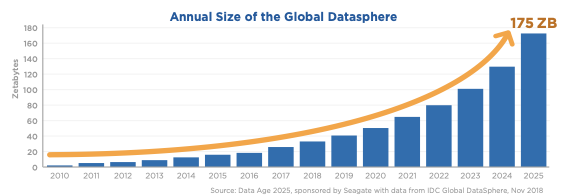
\includegraphics[width=0.8\textwidth]{Datasphere.png}
    \end{figure}
\end{frame}
%------------------------------------------------------

%------------------------------------------------------
\begin{frame}{Research Question}
    \begin{block}{Questions}
        - What are the effect of agents using data uncorrelated with fundamentals to forecast returns? \\
        - Are statistical tools enough to prevent equilibria non-consistent with rational expectations?
    \end{block}
\end{frame}
%------------------------------------------------------

%------------------------------------------------------
\begin{frame}{This paper}

\begin{itemize}
    \item Offers a rationale as to why agents might behave non-rationally \textbf{(cross-moment consistent equilibrium)}
    \item Analyzes different types of forecasting rules simple OLS, WLS with constant gain, LASSO regression
    \item Emprically tests the predictions of the model on multiple assets using the topic datasets of \textbf{Bybee et al. (2024)}
\end{itemize}

\end{frame}
%------------------------------------------------------

%------------------------------------------------------
\begin{frame}{Preview of Results}
\begin{itemize}
    \item Memory (gain) is crucial
    \item With decreasing gains (OLS) only cross-moment consistent equilibrium is REE 
    \item With constant gain (WLS) CMCE mean coincides with REE but distribution is different (excess volatilty)
    \item Lasso does not change the result and theoretically quanitify probability of window of predictabilities (returns being predictable because agents believe so based on their statistical tool)

\end{itemize}
\end{frame}
%------------------------------------------------------

\section{Current Status}

%------------------------------------------------------
\begin{frame}{Current Status}

\begin{itemize}
    \item Main theory is done (proofs being written up)
    \item Literature organized, needs to be incorporated into the paper
    \item Empirical analysis is ongoing
    \item Writing is ongoing
\end{itemize}

\end{frame}
%------------------------------------------------------

\section{Model Setup}

%------------------------------------------------------


%------------------------------------------------------
\begin{frame}{Baseline Framework}
\begin{itemize}
    \item Standard \textbf{Lucas (1978)} economy with a continuum of risk–neutral agents.
    \item One risky asset paying stochastic dividends \( D_t \).
    \item Dividends and consumption follow log–normal growth:
    \[
    \frac{D_t}{D_{t-1}} = a \varepsilon^d_t, 
    \quad
    \frac{C_t}{C_{t-1}} = a \varepsilon^c_t.
    \]
    \item Shocks:
    \[
    \begin{pmatrix}\log \varepsilon^d_t \\ \log \varepsilon^c_t \end{pmatrix}
    \sim \mathcal{N}\left(
    \begin{pmatrix} -s_d^2/2 \\ -s_c^2/2 \end{pmatrix},
    \begin{pmatrix} s_d^2 & \rho s_d s_c \\ \rho s_d s_c & s_c^2 \end{pmatrix}
    \right).
    \]
    \item Expected dividend growth: \( \mathbb{E}_t D_{t+1} = a D_t. \)
\end{itemize}
\end{frame}
%------------------------------------------------------

%------------------------------------------------------
\begin{frame}{Equilibrium Pricing under RE}
\begin{itemize}
    \item No–arbitrage condition:
    \[
    P_t = \delta \mathbb{E}_t \Big[\Big(\frac{C_{t+1}}{C_t}\Big)^{-\gamma}(P_{t+1}+D_{t+1}) \Big].
    \]
    \item Under rational expectations:
    \[
    P_t = \frac{\delta a^{1-\gamma}\rho_e}{1 - a^{1-\gamma}\rho_e} D_t,
    \quad
    \rho_e = e^{\gamma(1+\gamma)s_c^2/2 - \gamma\rho s_c s_d}.
    \]
    \item Price–dividend ratio constant.
    \item Gross return:
    \[
    R_{t+1} = \frac{P_{t+1}}{P_t} = a \varepsilon^d_{t+1}.
    \]
    \item Log–return: \( r_{t+1} = \log a + \log \varepsilon^d_{t+1} \).
\end{itemize}
\end{frame}
%------------------------------------------------------

%------------------------------------------------------
\begin{frame}{Adaptive Learning Setup}
\begin{itemize}
    \item Agents are \textbf{boundedly rational}: they estimate expected returns via econometrics.
    \item Perceived Law of Motion (PLM):
    \[
    r_{t+1} = x_t \beta + u_t, \quad x_t \sim \mathcal{N}(0, \sigma_x^2).
    \]
    \item Gross expected return:
    \[
    \mathbb{E}_t(R_{t+1}) = \phi e^{x_t \beta}, \quad \phi = e^{\sigma_u^2 / 2}.
    \]
    \item Plug into pricing equation:
    \[
    P_t = \frac{\delta a^{1-\gamma}\rho_e}{1 - \delta a^{-\gamma}\phi e^{x_t \beta}} D_t,
    \quad
    \kappa = \delta a^{-\gamma}\phi.
    \]
\end{itemize}
\end{frame}
%------------------------------------------------------

%------------------------------------------------------
\begin{frame}{Actual Law of Motion (ALM)}
\begin{itemize}
    \item From price dynamics:
    \[
    R_t = \frac{1 - \kappa e^{x_{t-1}\beta}}{1 - \kappa e^{x_t \beta}}\frac{D_t}{D_{t-1}}.
    \]
    \item Log form:
    \[
    r_{t+1} = \log \varepsilon_{t+1}
               + \log(1 - \kappa e^{x_t \beta})
               - \log(1 - \kappa e^{x_{t+1} \beta}).
    \]
    \item Nonlinear mapping between beliefs and realized returns $\Rightarrow$ PLM is misspecified.
    \item Agents update $\beta$ recursively $\Rightarrow$ stochastic recursive system.
\end{itemize}
\end{frame}
%------------------------------------------------------

%------------------------------------------------------
\begin{frame}{Cross-Moment Consistent Equilibrium}
\begin{itemize}
    \item Equilibrium condition:
    \[
    T(\beta) - \beta = 0, \quad
    T(\beta) = \frac{\text{Cov}(r_{t+1}, x_t)}{\text{Var}(x_t)}.
    \]
    \item Approximation (Taylor around $x_t=0$):
    \[
    \log(1 - \kappa e^{x_t\beta}) \approx 
    \log(1-\kappa) - \frac{\kappa}{1-\kappa}x_t\beta + \frac{\kappa}{2(1-\kappa)^2}(x_t\beta)^2.
    \]
    \item Then:
    \[
    T(\beta) \approx -\frac{\kappa}{1-\kappa}\beta
    \quad \Rightarrow \quad
    \beta^* = 0.
    \]
    \item Stable if \( \kappa < 1 \).
\end{itemize}
\end{frame}
%------------------------------------------------------

%------------------------------------------------------
\begin{frame}{Learning Algorithms}
\textbf{Recursive Least Squares (RLS):}
\[
\beta_t = \beta_{t-1} + t^{-1} S^{-1}_{t-1} x_{t-2}(r_{t-1}-x_{t-2}\beta_{t-1}),
\quad
S_t = S_{t-1} + t^{-1}(x_{t-2}^2 - S_{t-1}).
\]
\begin{itemize}
    \item Fits canonical stochastic recursive algorithm form.
    \item Stability $\Leftrightarrow$ ODE 
    \( \frac{d\beta}{d\tau} = T(\beta)-\beta \).
\end{itemize}
\vspace{0.5em}
\textbf{Constant-Gain (WLS):}
\[
b_t = b_{t-1} + \gamma M_t^{-1}x_t(y_t - x_t b_{t-1}),
\]
\begin{itemize}
    \item Gain $\gamma \in (0,1)$ constant $\Rightarrow$ perpetual fluctuations.
    \item Stationary distribution:
    \[
    \beta_t \sim \mathcal{N}\left(0,\, \gamma s_d^2 [2\sigma_x^2(1+\tfrac{\kappa}{1-\kappa})]^{-1}\right).
    \]
\end{itemize}
\end{frame}
%------------------------------------------------------

%------------------------------------------------------
\begin{frame}
    \frametitle{LASSO Learning and Implications}
   \begin{itemize}
    \item Agents use LASSO estimator:
    \[
    {\beta}_{LASSO}
    = \text{sign}(\beta_{OLS})\max(0,|\beta_{OLS}| - \lambda).
    \]

    \item Mapping: \( \beta_{OLS} = -\frac{\kappa}{1-\kappa}\beta_{LASSO}. \)
    \item Only $\beta^*=0$ stable for $\kappa<1$.
    item Probability of nonzero estimate:
    \[
    \mathbb{P}(|\beta_{OLS}|>\lambda)
    = 1 - [\Phi(\lambda/\sigma_{OLS}) - \Phi(-\lambda/\sigma_{OLS})].
    \]
    
\end{itemize}

\end{frame}
%------------------------------------------------------

\section{Emprical Application}

%------------------------------------------------------
\begin{frame}{Empirical Application}
Theory suggests using a two stage approach:
\begin{itemize}
    \item Stage 1: Run mis-specified regression implied by PLM on log-returns to recover agents' beliefs
    \begin{equation}
    r_{t+1} = X_t \beta + u_{t+1},
    \end{equation}
    where \( X_t \) is a large set of predictors uncorrelated with dividends.
    \item Stage 2: Estimate the non-linear ALM implied by agents' beliefs.
    \begin{equation}
    r_{t+1} = \log \varepsilon_{t+1}
               + \log(1 - \kappa e^{X_t \beta})
               - \log(1 - \kappa e^{X_{t+1} \beta}).
    \end{equation}
\end{itemize}
\end{frame}
%------------------------------------------------------

%------------------------------------------------------
\begin{frame}{Computational Challenges}
Stage 1 is driven by choice of:
\begin{itemize}
    \item Window size (Gain)
    \item Regularization parameter (LASSO)
    \item Frequncy (Daily, Weekly, Monthly)
\end{itemize}

\begin{block}{Problem}
    Thoery predicts that stage 1 is mis-specified. 
    If we optimize routine for stage 1 fit we impose bad fit for stage 2.
    
\end{block}

\begin{block}{Solution}
    Use cross-validation to choose parameters that optimize stage 2 fit.
    But \textbf{computanally expensive.}
\end{block}
\end{frame}

\end{document}
